\section{Modelo de TRFs por regresión regularizada}
\label{sec:modelo_regresion}

% Describir cómo se incorporan las features al modelo de regresión EEG.
% Explicar la estrategia de construcción incremental:
% partir del mejor modelo base, agregar features de a una,
% seleccionar las que sobreviven, luego agregar interacciones.
% Justificar la estrategia.

El objetivo principal de esta tesis es investigar si las features \todo{o variables, renombrar} extraídas del modelo nnELM tienen correlatos con la actividad neural. El análisis de la actividad cerebral durante las tareas de búsqueda visual tiene una dificultad particular: las respuestas cerebrales de fijaciones sucesivas se solapan temporalmente. La duración típica de una fijación presenta una media de 219ms, un tiempo considerablemente menor a la ventanal temporal necesaria para capturar una respuesta completa, la cual se extiende a lo largo de 600ms. \todo{cita}

\subsection{Temporal Response Functions (TRFs)}

Una Temporal Response Function (TRF) es la respuesta neural estimada asociada a un predictor específico en función del tiempo relativo al onset del evento.  Para cada variable del modelo, la TRF es una curva que indica cuánto varía la señal EEG en cada retardo temporal ante un cambio unitario de ese predictor: si la TRF de un predictor muestra un pico positivo a los 300ms, significa que en promedio la señal EEG aumenta 300ms después de que ese evento ocurre. De esta manera, el conjunto de TRFs del modelo describe cómo cada variable de interés modula la actividad cerebral a lo largo del tiempo.

\subsection{Construcción de Matriz de Diseño}

El framework de TRFs por Regresión Regularizadas \todo{cita} representa la señal EEG de cada electrodo como una combinación lineal de las respuestas a distintos tipos de eventos. Por ejemplo, para un solo predictor $x$ con ventana de $L$ lags:

\begin{equation}
r(t) = \sum_{\tau=0}^{L} w(\tau) \cdot x(t - \tau) + \varepsilon(t)
\end{equation}

donde $r(t)$ es la señal EEG en el instante $t$; $x(t-\tau)$ es el valor del predictor $\tau$ muestras antes; $w(\tau)$ son los coeficientes que se quieren estimar (la TRF) y $\epsilon(t)$ es el error residual. La TRF es la secuencia de coeficientes $w(\tau)$ para cada lag $\tau$.

Para cada participante se construye una matriz de diseño M que codifica, para cada muestra temporal de la señal EEG continua, qué eventos ocurrieron en una ventana temporal definida. 

Cada columna de M corresponde a un predictor desplazado en el tiempo (llamado lag). En otras palabras, para cada variable de interés y cada retardo temporal dentro de la ventana, se incluye una columna que indica el valor de esa variable en ese retardo.

\begin{table}[h]
\centering
\small
\begin{tabular}{c|ccc|ccc|ccc}
\toprule
 & \multicolumn{3}{c|}{\texttt{variable\_1} (binaria)} & \multicolumn{3}{c|}{\texttt{variable\_2} (binaria)} & \multicolumn{3}{c}{\texttt{variable\_3} (continua)} \\
 & $\tau_0$ & $\tau_1$ & $\tau_2$ & $\tau_0$ & $\tau_1$ & $\tau_2$ & $\tau_0$ & $\tau_1$ & $\tau_2$ \\
\midrule
$t_1$ & 1 & 0 & 0 & 0 & 0 & 0 & 0.8 & 0.0 & 0.0 \\
$t_2$ & 0 & 1 & 0 & 0 & 0 & 0 & 0.0 & 0.8 & 0.0 \\
$t_3$ & 0 & 0 & 1 & 1 & 0 & 0 & 0.0 & 0.0 & 0.8 \\
$t_4$ & 0 & 0 & 0 & 0 & 1 & 0 & 0.0 & 0.0 & 0.0 \\
$t_5$ & 1 & 0 & 0 & 0 & 0 & 1 & 0.3 & 0.0 & 0.0 \\
\bottomrule
\end{tabular}
\caption{Ejemplo simplificado de la matriz de diseño $\mathbf{M}$ para tres predictores y una ventana de 3 lags. Cada fila corresponde a una muestra temporal de la señal EEG continua. Las variables binarias toman valor 1 en el onset del evento y se desplazan diagonalmente con cada lag. La variable continua refleja el valor del predictor en ese retardo.}
\label{tab:matriz_disenio}
\end{table}

\subsection{Estimación Ridge y selección del parámetro de regularización}

Los coeficientes del modelo (las TRFs) se estiman metiante regresión Ridge (regularización L2).

\begin{equation}
\hat{\mathbf{w}} = \arg\min_{\mathbf{w}} \left[ \sum_t \left( r(t) - \sum_{\tau} w(\tau) \cdot x(t-\tau) \right)^2 + \lambda \sum_{\tau} w(\tau)^2 \right]
\end{equation}

El primer término corresponde al error de predicción: qué tan bien el modelo explica la señal EEG observada. El segundo término es la penalización Ridge, que encoge los coeficientes hacia cero y está controlada por el parámetro $\lambda$. Esta penalización estabiliza la estimación en presencia de multicolinealidad entre predictores y previene el sobreajuste.

\subsubsection{Selección de $\lambda$}

El parámetro $\lambda$ se selecciona individualmente para cada participante y modelo mediante la técnica de \textit{cross-validation} de 10 folds. En cada iteración, el modelo se entrena sobre el 90\% de los datos para un conjunto de valores candidatos 
de $\lambda$, y se evalúa sobre el 10\% restante midiendo el coeficiente de correlación 
de Pearson entre la señal EEG predicha y la señal real. El $\lambda$ óptimo es aquel 
que maximiza la correlación promedio entre los 10 folds.

\subsubsection{El modelo base: MD2}

Cómo punto de partida para el análisis, se adopta el modelo base MD2 definido en \todo{cita}, que incluye los siguientes predictores:

\begin{itemize}
    \item \textbf{Intercept de fijación}: respuesta media asociada a cualquier 
    fijación sobre un estímulo.
    \item \textbf{Target}: variable binaria que indica si la fijación cayó sobre 
    el target (1) o un distractor (0).
    \item \textbf{Memory Set Size (MSS)}: tamaño del conjunto de memoria, 
    codificado ordinalmente como $\{0, 1, 3\}$ para MSS $\in \{1, 2, 4\}$.
    \item \textbf{Correct}: variable binaria que indica si el participante 
    respondió correctamente en ese trial.
    \item \textbf{Intercept de sacada}: respuesta media asociada a cada 
    movimiento sacádico.
    \item \textbf{Splines de amplitud de sacada}: 5 splines cúbicos que 
    modelan la relación no lineal entre la amplitud de la sacada y la 
    respuesta EEG.
\end{itemize}

La ventana de análisis se define entre $-200$ ms y $+400$ ms respecto al onset 
de cada fijación, y entre $-200$ ms y $+400$ ms respecto al onset de cada sacada.


\subsection{Interpretación de las TRFs: regiones cerebrales y componentes de referencia}

Las TRFs estimadas por el modelo producen patrones de actividad
con una estructura espacial y temporal específica: actividad neuronal
que ocurre a latencias determinadas y que se concentra en
regiones particulares del cuero cabelludo. Para poder interpretar
esos patrones en la sección de Resultados, esta sección introduce
los conceptos básicos de neurociencia necesarios: la organización
espacial de los electrodos EEG y los componentes neurales de
referencia que se pueden observar tanto en el modelo base como en los experimentos realizados.

La señal EEG se registra simultáneamente en múltiples electrodos
distribuidos sobre el cuero cabelludo. Esta distribución espacial permite localizar aproximadamente
qué región cortical genera cada respuesta: los electrodos frontales (ubicados en la parte delantera 
de la cabeza) reflejan procesos cognitivos de alto nivel como
planificación, control atencional y memoria de trabajo;
los electrodos parietales (ubicados en la parte 
trasera) capturan procesos de atención espacial; los electrodos occipitales (ubicados 
en la parte de atrás de la cabeza) capturan principalmente actividad 
de la corteza visual primaria, reflejando el procesamiento visual 
temprano ante cada fijación.


\begin{figure}[H]
    \centering
    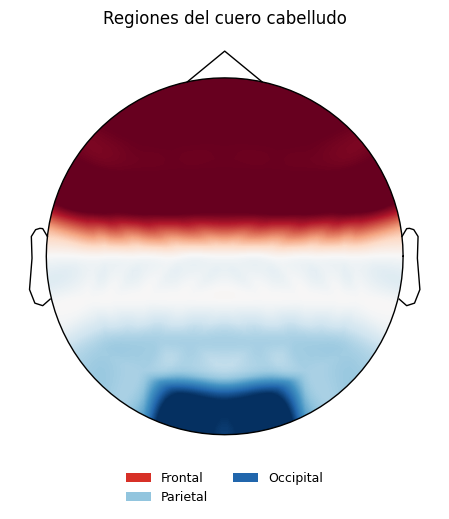
\includegraphics[width=0.3\textwidth]{chapters/02_materiales_metodos/images/cabecita_regiones.png}
    \caption{Distribución de las regiones del cuero cabelludo según 
su ubicación anatómica.}
    \label{fig:regiones_corteza}
\end{figure}


La respuesta neural ante un evento puede caracterizarse a través de
\textit{componentes}: patrones de activación de la señal EEG que
ocurren a latencias específicas tras el onset del evento y que están
bien establecidos en la literatura de neurociencia cognitiva. Por
convención, los componentes se nombran según la polaridad de la
activación (positiva (P) o negativa (N)) y su latencia aproximada
en milisegundos. Por ejemplo, el P100 es una activación positiva
que ocurre alrededor de los 100 ms; el N200, una activación negativa
alrededor de los 200 ms.

El \textbf{compontente P100} es un componente positivo temprano 
que ocurre entre los 80 y 130 ms tras la presentación de un 
estímulo visual, con distribución sobre electrodos occipitales 
laterales. Refleja el procesamiento visual temprano ante la llegada de ueva información visual. El P100 puede ser modulado por la atención: su  amplitud aumenta cuando el estímulo aparece en una región del 
campo visual que el sujeto estaba atendiendo.  

El \textbf{componente P300} es un componente positivo tardío que ocurre entre los 
250 y 500 ms tras el onset de un estímulo, con pico típico 
alrededor de los 300 ms y distribución máxima sobre electrodos 
parietales. A diferencia del P100, su ocurrencia no depende de las características físicas del 
estímulo sino de la relevancia que ese estímulo tiene para 
la tarea en curso. En particular, el P300 se asocia a procesos 
de evaluación y categorización del estímulo.